% Created 2023-10-06 vie 00:12
% Intended LaTeX compiler: pdflatex
\documentclass[11pt]{article}
\usepackage[utf8]{inputenc}
\usepackage[T1]{fontenc}
\usepackage{graphicx}
\usepackage{grffile}
\usepackage{longtable}
\usepackage{wrapfig}
\usepackage{rotating}
\usepackage[normalem]{ulem}
\usepackage{amsmath}
\usepackage{textcomp}
\usepackage{amssymb}
\usepackage{capt-of}
\usepackage{hyperref}
\usepackage{../modern}
\bibliography{./sources.bib}
\raggedbottom
\setcounter{secnumdepth}{2}
\author{Luis Eduardo Galindo Amaya (1274895)}
\date{25 de Septiembre 2023}
\title{Meta 3.1 - Conocer e identificar}
\hypersetup{
 pdfauthor={Luis Eduardo Galindo Amaya (1274895)},
 pdftitle={Meta 3.1 - Conocer e identificar},
 pdfkeywords={},
 pdfsubject={},
 pdfcreator={Emacs 27.1 (Org mode 9.3)}, 
 pdflang={Spanish}}
\begin{document}

\modentitlepage{../images/escudo-uabc-2022-color-cont.png}
\tableofcontents
\pagebreak
\datasection{Individual}

\section{Realizar un mapa conceptual}
\label{sec:org651c497}
\begin{center}
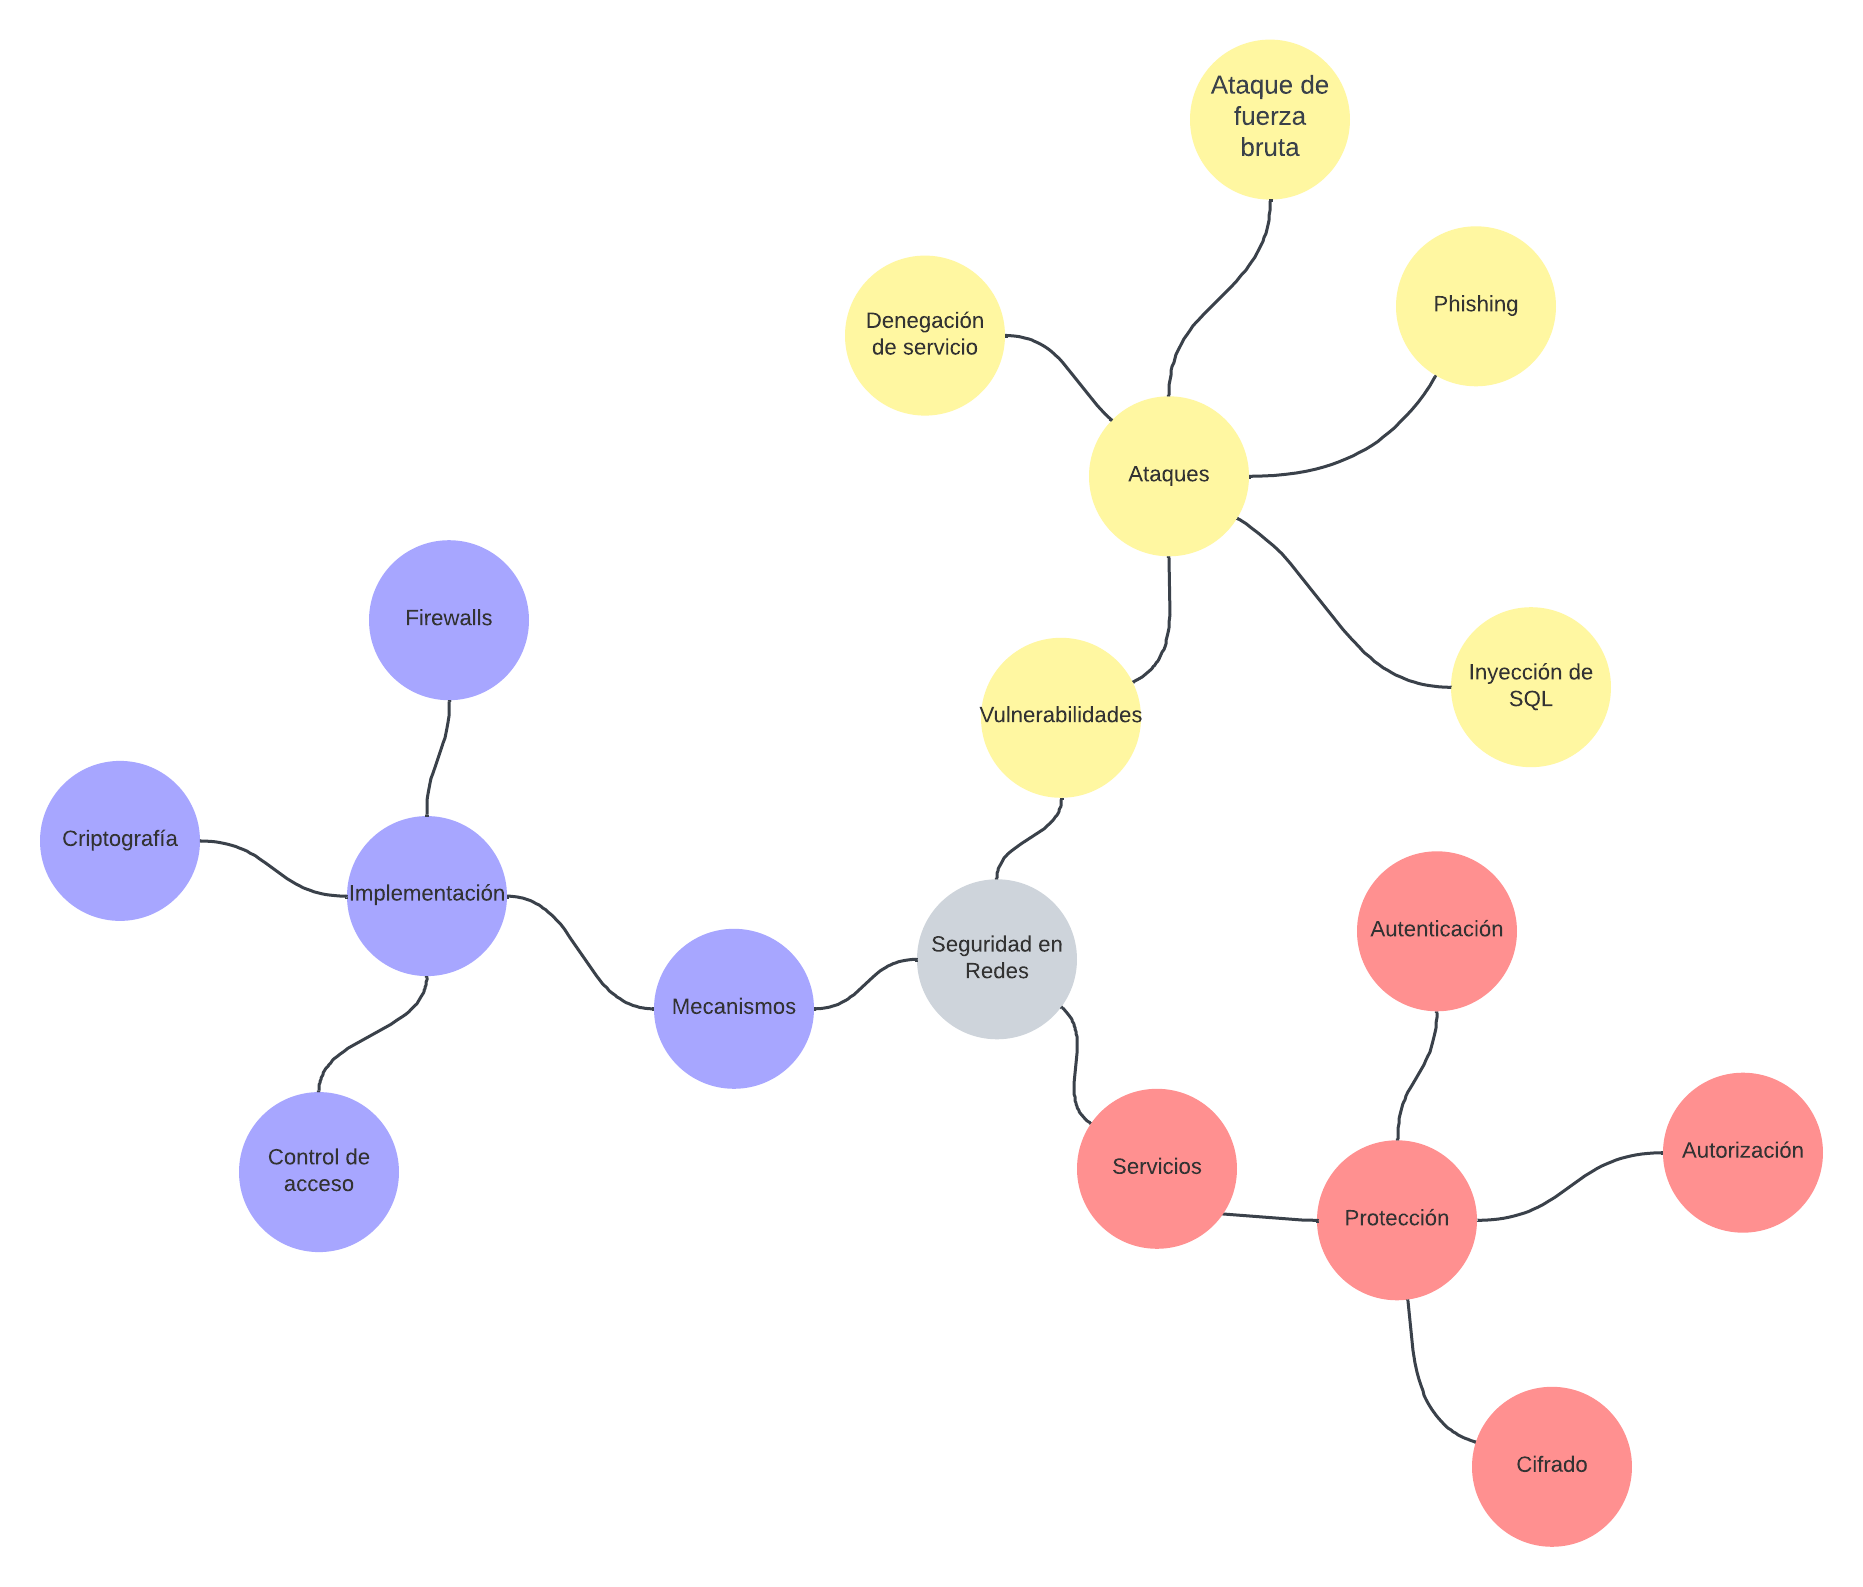
\includegraphics[width=.9\linewidth]{Mapa mental.png}
\end{center}

\cite{Stallings}

\section{Modelo de seguridad}
\label{sec:org2eaadda}
Un modelo de seguridad es un conjunto de reglas, politicas y procedimientos que 
se implementan en una red para proteger la integridad, privacidad y el accesos
a los recursos, el modelo de seguridad en redes nos permite garantizar la 
seguridad de la red y reducir las amenazas, los ataques cibernéticos y las 
actividades maliciosas. \\


Una adecuado modelo de seguridad permite a toda una organizacion acceder de 
manera segura a los recursos sin exponer a los demas usuarios y eliminar o al 
menos mitigar los daños que puedan ser provocado por agentes externos. \\


Un modelo de seguridad esta compuestos de diferentes medidas como 
Políticas de seguridad, Autenticación, Firewalls, Cifrado etc, aun así es 
nesesario actualizar los modelos de seguridad constantemente la seguridad 
actualmente es uno de los fatores mas criticos de una organizacion de cualquier
tipo.

\section{Conclusión}
\label{sec:org4c0e50b}
A lo largo de esta practica pude aprender que son ataques, servicios, mecanismos 
y como un modelo de seguridad puede lograr que la red sea más segura utilizando 
medidas preventivas de seguridad.


\section{Referencias}
\label{sec:org959170a}
\printbibliography[heading=none]
\end{document}
